\begin{figure}[t]
    \centering
    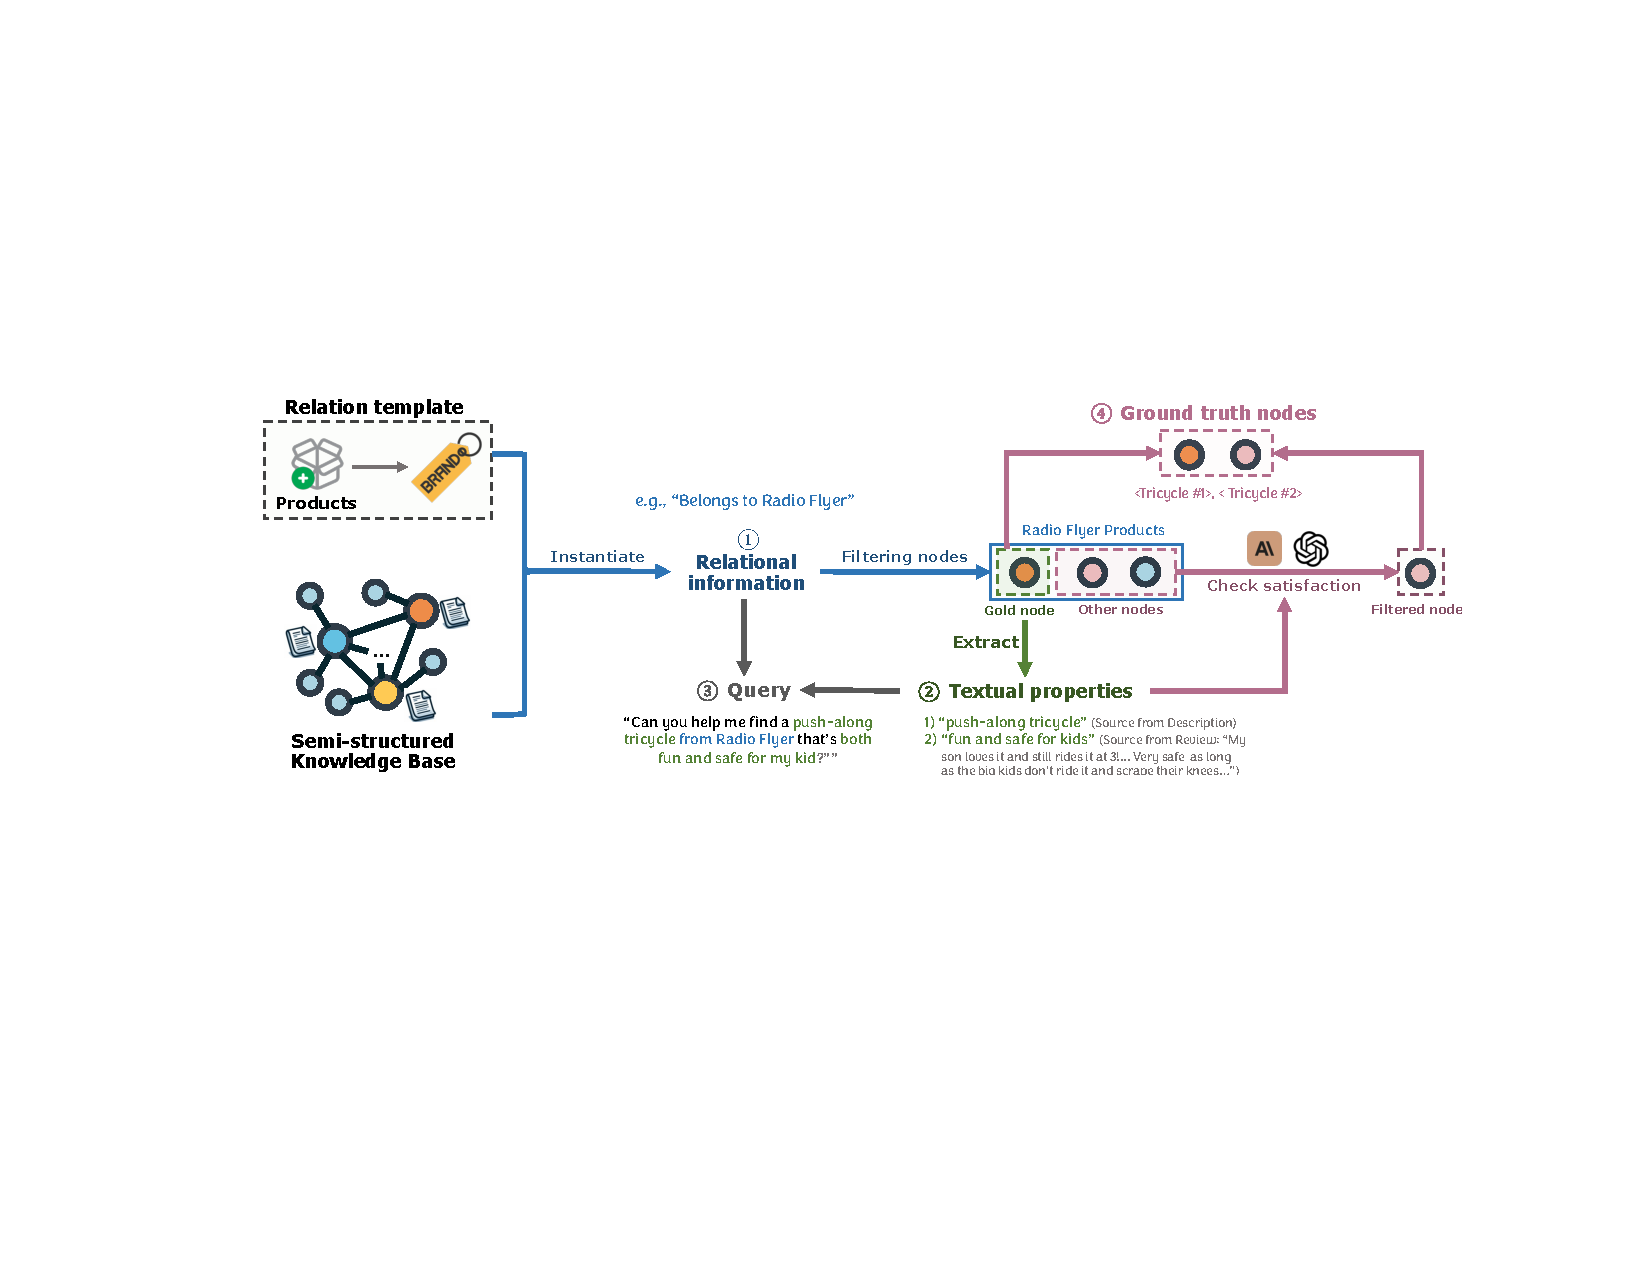
\includegraphics[width=0.95\textwidth]{figs/construction}
    \vspace{-3pt}
    \caption{
    The construct pipeline to generate our semi-structured retrieval datasets.
    % involves four main steps: 1) Sample Relational Requirement: Based on relational templates, sample a relational requirement on a SKB.
    % 2) Extract Textual Properties: From a node that meets the relational requirement, extract relevant textual properties.
    % 3) Combine Information: Merge the relational information and textual properties to form a natural-sounding query.
    % 4) Construct Ground Truth Nodes: Check if nodes satisfy the textual properties using multiple language models to establish ground truth nodes.
    }
    \vspace{-10pt}
    %\kexin{what is the meaning of edge color?}
    %\shirley{the edge colors are made the same as the arrow color}
    \label{fig:construction}
\end{figure}

\vspace{-2pt}
\subsection{Benchmark Construction: Synthesized Queries} 
\label{sec:construction}
\vspace{-2pt}
% \karthik{this section needs a running example and should be tied closely to the numbering in Fig 5}
In Figure~\ref{fig:construction}, we present a novel pipeline that synthesizes the SKB queries and automatically generates the ground truth answers. 
The key idea is to entangle relational and textual information during synthesis and disentangle them during answer filtering. 
It involves four steps as follows:
% The pipeline involves four steps and the specific processes vary depending on the characteristics of each dataset. These steps are as follows:

% We leverage the GPT and Claude language models to construct the retrieval datasets. Detailed descriptions of all the prompts we used are available in Appendix~\ref{app:prompts}. 

\begin{itemize}[leftmargin=*]
\vspace{-2pt}
\item \textbf{1) Sample Relational Requirements:} For each query, we sample a practical relation template constructed with expert/domain knowledge, \eg ``\texttt{(a product) belongs to <brand>}'' and ground it with sampled entities (\ie a specific brand), \eg ``belongs to Radio Flyer''. 
This relational requirement yields a set of candidate entities, \ie products belonging to Radio Flyer. 
% \revision{The relation templates for the three SKBs are practical and constructed with expert/domain knowledge}, which are available in Appendix~\ref{app:details}. 
% Therefore, we obtain the relational requirements and the corresponding candidates. 
% For instance, the template ``What is the drug that targets the genes or proteins which are expressed in <anatomy>?'' is particularly valuable for precision medicine inquiries. It aids in pinpointing medications aimed at specific genetic or protein targets within defined anatomical areas, thereby contributing to the development of targeted treatments. 
% \shirley{relate text to figure, \eg step 1}
\vspace{-2pt}
\item \textbf{2) Extracting Textual Properties:} \revision{
% The relational requirement yields a set of satisfying candidates. 
We randomly sample a candidate entity from the first step, referred to as the \textit{gold answer}, from which LLMs extract properties that align with the interests of specific roles (\eg customers, researchers, or doctors) in its textual document}.  In Figure~\ref{fig:construction}, we extract multiple properties about the functionality and user experience from a Radio Flyer product. 
%%%%%% We utilize GPT-3.5-turbo-16k for the \amazonh and Claude-v2 for the other two datasets to conduct this step, where the prompts used are included in Appendix~\ref{app:prompts}.  
% \karthik{how?}
\vspace{-2pt}
\item \textbf{3) Combining Textual and Relational Information:} 
We use two LLMs to synthesize queries from textual properties and relational requirements, enhancing diversity and reducing bias arise from relying on a single LLM. 
The first LLM focuses on generating natural, role-specific, and style-consistent (\eg ArXiv searches) queries. The second LLM enriches the context and rephrases queries, which poses the need for advanced reasoning to comprehend them under complex contexts.

\vspace{-2pt}
\item \textbf{4) Filtering Additional Answers:} 
Finally, we employ multiple LLMs to verify if the candidates from the first step meet the extracted textual properties. Only candidates passing all LLM verifications are included in the final ground truth set. To assess the precision of this filtering mechanism, we compute the average ratios for the gold answers to be verified, which are 86.6\%, 98.9\%, and 92.3\% on the three datasets, highlighting our efficacy in yielding high-quality ground truth answers.

\vspace{-2pt}
\end{itemize}

This dataset construction pipeline is automatic, efficient, and broadly applicable to the SKBs in our formulation.  
\revision{We include all of the prompts and the LLMs versions in the above steps in Appendix~\ref{app:prompts}.} 
